\documentclass[a4paper,10pt]{article}

\usepackage{amsmath}
\usepackage{amstext}
\usepackage{amssymb}
\usepackage{amsfonts}
\usepackage{amsthm}
\usepackage{etoolbox}
%mathspec/fontspec
\usepackage{mathspec}
\usepackage{xunicode}
\usepackage{xltxtra}

\usepackage[bookmarks,bookmarksnumbered]{hyperref}

\makeatletter       % changes [1] to 1. in bibliography
\renewcommand{\@biblabel}[1]{#1.}
\makeatother

\usepackage{appendix}
\usepackage{graphicx}
\usepackage{natbib}


% FONT
\setmainfont[Mapping=tex-text,Numbers={Lining}]{Linux Libertine O}
\setmathfont(Latin)[Numbers={Lowercase}]{Linux Libertine O}
\setmathfont(Digits)[Scale=MatchLowercase]{Linux Libertine O}

\usepackage{unicode-math}
\setmainfont[Mapping=tex-text,Numbers={Lining}]{Linux Libertine O} 
\setmathfont{XITS Math}

\setmathfont[range={\mathup}]{Linux Libertine O} 
\setmathfont[range={\mathit}]{Linux Libertine O Italic} 
\setmathfont[range={\rm}]{Linux Libertine O} 
\setmathfont[range={\mathrm}]{Linux Libertine O} 



% \renewcommand{\rmdefault}{fxl}
\renewcommand{\sfdefault}{txss}


%%%%%%%%% from here yuasa setting %%%%%%%%%%%%%%%%%%%%%
% a4paper paperheight = 845.04684pt
%\setlength{\topmargin}{-.5in}
%% textheight = paperheight - 2in - \topmargin - \headheight - \headsep
%%              - \footskip = approx. 641pt
%\setlength{\textheight}{1.05\paperheight}
%\addtolength{\textheight}{-2.2in}
%%\addtolength{\textheight}{-\topmargin}
%%\addtolength{\textheight}{-\headheight}
%%\addtolength{\textheight}{-\headsep}
%%\addtolength{\textheight}{-\footskip}

%% a4paper paperwidth = 597.50787pt
%%\setlength{\marginparsep}{0pt}
%%\setlength{\marginparwidth}{0pt}
%% textwidth = paperwidth - 2in - \oddsidemargin = approx. 432pt
%\setlength{\textwidth}{\paperwidth}
%\addtolength{\textwidth}{-1.8in}
%%\addtolength{\textwidth}{-\oddsidemargin}

%% add 20pt to sidemargin
%%   oddside: 1in+20pt+20pt | \textwidth | 1in-20pt
%%   evenside: 1in-20pt | \textwidth | 1in+20pt+20pt
%\setlength{\oddsidemargin}{0pt}
%\setlength{\evensidemargin}{0pt}

%%%%%%%%% to here yuasa setting %%%%%%%%%%%%%%%%

%%%%%%%%% from here margin setting %%%%%%%%%%%%%%%%
%for dron
%\setlength{\topmargin}{0pt}
%\setlength{\marginparsep}{0pt}
%\setlength{\marginparwidth}{0pt}
%\setlength{\oddsidemargin}{20pt}
%\setlength{\evensidemargin}{0pt}
%
%\setlength{\textwidth}{\paperwidth}
%\addtolength{\textwidth}{-2in}
%\addtolength{\textwidth}{-\oddsidemargin}
%
%\addtolength{\oddsidemargin}{0pt}
%\addtolength{\evensidemargin}{-23pt}
%\setlength{\topmargin}{-12mm}
%\setlength{\textheight}{25.3cm}
%\setlength{\textwidth}{16.3cm}
%%%%%%%%% till here margin setting %%%%%%%%%%%%%%%%

%%% Linestrech
%for user guide
\renewcommand{\baselinestretch} {1.1}
%for dron
%\renewcommand{\baselinestretch} {1.1}

\setlength\bibsep{2pt}
\renewcommand{\bibnumfmt}[1]{(#1)}


%%% Table of Contents
\usepackage{tocloft}
\setlength\cftparskip{-0.7pt}
\setlength\cftbeforesecskip{1.5pt}
\setlength\cftaftertoctitleskip{2pt}

\addtolength{\oddsidemargin}{-.875in}
	\addtolength{\evensidemargin}{-.875in}
	\addtolength{\textwidth}{1.75in}

	\addtolength{\topmargin}{-.875in}
	\addtolength{\textheight}{1.75in}

%% for quotes
%\fontspec[Mapping=tex-text]{Linux Libertine O}
%\fontspec[Ligatures=TeX]{Linux Libertine O}

%%%%%%%%% color %%%%%%%%%
\usepackage{color}
\newcommand{\red}{\textcolor{red}}
\newcommand{\green}{\textcolor{green}}
\newcommand{\blue}{\textcolor[rgb]{0,0,0.8}}
\newcommand{\midnightblue}{\textcolor[rgb]{0.0976,0.0976,0.4375}}
\newcommand{\apricot}{\textcolor[rgb]{1,0,0.5}}
\newcommand{\strawberry}{\textcolor[rgb]{1,0,0.5}}
\newcommand{\orange}{\textcolor[rgb]{0.949, 0.593, 0}}
\newcommand{\gray}{\textcolor[rgb]{0.4,0.4,0.4}}
%%%%%%%%%%%%%%%%%%%%%%%%%%%


%%%%%%%%% for source code listing %%%%%%%%%
\usepackage{listings}


\lstset{%
 language={XML},
 backgroundcolor={\color[gray]{.97}},%
 basicstyle={\small\ttfamily},%
% identifierstyle={\small\ttfamily},%
 commentstyle={\gray},%
% keywordstyle={\small\bfseries\ttfamily},%
% ndkeywordstyle={\small},%
% stringstyle={\apricot},
 frame={tb},
 breaklines=true,
% columns=[l]{fullflexible},%
 numbers=left,%
% xrightmargin=5pt,%
% xleftmargin=5pt,%
% numberstyle={\scriptsize},%
% stepnumber=1,
 numbersep=5pt,%
 lineskip=-0.5pt,%
 showstringspaces=false,
 numbers=none
}
%%%%%%%%%%%%%%%%%%%%%%%%%%%

\title{\Huge{
SpaceWire RMAP Library v2}\\
\Large{User Guide}}

\author{
{\Large
Takayuki Yuasa
}\\
{\small Japan Aerospace Exploration Agency, Institute of Space and Astronautical Science}\\
{\small yuasa \_at\_mark\_ astro.isas.jaxa.jp}
}

\date{January 10,  2012}


\begin{document}
\maketitle
{\small
\tableofcontents
}
\setcounter{page}{2}

%%%%%%%%%%%%%%%%%%%%%%%%%%%%%%%%%%%%%%
%%%%%%%%%%%%%%%%%%%%%%%%%%%%%%%%%%%%%%
\section{Overview of SpaceWire RMAP Library}\label{section:overview}
SpaceWire RMAP Library is an open-source C++ class library for developments and tests of SpaceWire\footnote{ECSS-E-ST-50-12C.} networks and data transfer over RMAP\footnote{Remote Memory Access Protocol. ECSS-E-ST-50-52C.}. The library is highly modularized, and provides easy-to-use access to SpaceWire interfaces and a software RMAP stack.

The SpaceWireIF class abstracts a physical SpaceWire interface, and an implementation class for SpaceWire-over-TCP interface is implemented as SpaceWireIFOverTCP. RMAP initiator and target functions can be multiplexed on a single SpaceWire interface, and the RMAPEngine class acts as a central engine for RMAP-related activities. RMAP target node information such as a target logical address, a target SpaceWire address, key, and so on, are managed via XML-like configuration files making it easier to handle multiple target nodes in a large SpaceWire network.

SpaceWire RMAP Library can be used on Mac OS X and Linux (probably with slight modification), and perhaps Windows with the Cygwin environment. If anyone ports the library to Windows, feedback the resulting source tree.
SpaceWire RMAP Library uses libraries listed below:
\begin{itemize}
  \setlength{\parskip}{0cm}
  \setlength{\itemsep}{0cm}
\item CxxUtilities\footnote{\url{https://github.com/yuasatakayuki/CxxUtilities}}
\item XMLUtilities by Soki Sakurai from The University of Tokyo\footnote{\url{https://github.com/sakuraisoki/XMLUtilities/}}
\item xerces-c++ by the Apache project\footnote{\url{http://xerces.apache.org/xerces-c/}\label{url:xerces}}
\end{itemize}
Among these, CxxUtilities and XMLUtilities are header-only libraries, and and xerces-c++ should be built before using SpaceWireRMAPLibrary.

Note that the software is distributed for free assuming that this is useful for some users without any warranty or official support, and developers are not responsible for any damages caused by this software.

\subsection{Changes from SpaceWire RMAP Library v1}
In 2006, SpaceWire RMAP Library v1 was released, and has been used in many applications and in many institutes.
Since RMAP was in a drafting phase at that time, the RMAP implementation in v1 was tentative, and is now obsolete in many ways (e.g. naming convention).
SpaceWire RMAP Library v2 which was written from scratch totally replaces v1, with many new functions which improves flexibility and controllability of SpaceWire and RMAP functions.

The SpaceWire RMAP Library v1 code is still contained in the v2 folder so as to allow old users to work with their applications developed for v1 (see SpaceWireRMAPLibrary/classic/). However, maintenance to the v1 code is suspended, and development power is devoted to v2.

%%%%%%%%%%%%%%%%%%%%%%%%%%%%%%%%%%%%%%
%%%%%%%%%%%%%%%%%%%%%%%%%%%%%%%%%%%%%%
\section{About this user guide}
The user guide is provided {\it as is} expecting that this is somewhat useful for users to use the software. This is a voluntary mission, and therefore, kind help is always welcome. It is greatly appreciated to make contributions by feed-backing comments, revising documents, and so on.

One of the Japanese authors of this document, Takayuki Yuasa, is sorry for his limited English capability, and will be very happy if anyone can help to improve it. Comments on grammar, vocabularies, phrasing, and composition are welcome!

\subsection{Latest information and feedback}
Latest information on SpaceWire RMAP Library can be found at the open-source SpaceWire project website \footnote{The open-source SpaceWire project: \url{https://galaxy.astro.isas.jaxa.jp/~yuasa/SpaceWire}\label{url:supportpage}}.

\subsection{References}
Documents listed below can be a nice reference when better understanding SpaceWire RMAP Library. Some of the documents can be obtained from the open-source SpaceWire project website$^\mathrm{\ref{url:supportpage}}$.
\begin{itemize}
  \setlength{\parskip}{0cm}
  \setlength{\itemsep}{0cm}
\item SpaceWire-to-GigabitEther User Guide
\item SpaceWire RMAP GUI User Guide
\item ECSS-E-ST-50-12C - "SpaceWire - Links, nodes, routers and networks" by ECSS
\item ECSS-E-ST-50-52C "SpaceWire - Remote memory access protocol" by ECSS
\end{itemize}

\subsection{Revisions}
\begin{itemize}
  \setlength{\parskip}{0cm}
  \setlength{\itemsep}{0cm}
\item 2012-01-10 Takayuki Yuasa. First release.
\end{itemize}



%%%%%%%%%%%%%%%%%%%%%%%%%%%%%%%%%%%%%%
%%%%%%%%%%%%%%%%%%%%%%%%%%%%%%%%%%%%%%
\section{Download, install, and compile with user applications}\label{section:downloadAndSettings}
SpaceWire RMAP Library is distributed as a zip archive at the open-source SpaceWire project website.
Git repository can be cloned from the github page\footnote{\url{https://github.com/yuasatakayuki/SpaceWireRMAPLibrary}}. 
Since SpaceWire RMAP Library is a header-only library, installation is simple; unzip the archive, and then move SpaceWireRMAPLibrary folder to wherever you like. Possible locations are for example /Users/{\it username}/Documents/workspace/SpaceWireRMAPLibrary, /Users/{\it username}/install/SpaceWireRMAPLibrary, or /usr/local/SpaceWireRMAPLibrary.

After installing the library, an environmental variable �gSPACEWIRERMAPLIBRARY\_PATH�h should be set to point the installed folder to simplify Makefiles used when compiling user applications. In the shell initialization file (.zshrc for zsh, and .bashrc for bash), add a line below:
\lstset{language=C++}
\begin{lstlisting}[label=source:sample_for_ssdtp2, caption=Sample code for filling the size and the data sections.]
export SPACEWIRERMAPLIBRARY_PATH=/Users/yuasa/workspace/SpaceWireRMAPLibrary
\end{lstlisting}
Change the path to match your install location.

The library uses several other libraries as mentioned in \S\ref{section:overview}.
Install xerces-c++ by downloading its source archive from the project page$^\mathrm{\ref{url:xerces}}$.
An example Makefile distributed with SpaceWire RMAP Library uses an environmental variable "XERCESDIR".
Set "XERCESDIR" in the shell initialization file, e.g.
\lstset{language=C++}
\begin{lstlisting}[label=source:sample_for_ssdtp2, caption=Sample code for filling the size and the data sections.]
export XERCESDIR=/Users/yuasa/work/install/xerces-c-3.1.1
\end{lstlisting}

Although CxxUtilities and XMLUtilities are also required by SpaceWire RMAP Library, a release version of SpaceWire RMAP Library includes these libraries for users' convenience; in SpaceWireRMAPLibrary/externalLibraries/.
Therefore, by default, environmental variables for these libraries are automatically set in an example Makefile, and users do not need to redefine them.
If a user wants to use their own installation(s) of CxxUtilities and/or XMLUtilities, set "CXXUTILITIES\_PATH" and "XMLUTILITIES\_PATH" reflecting his/her environment.

Table \ref{table:environmentalVariables} lists environmental variables used by SpaceWire RMAP Library Makefile. List \ref{source:sample_Makefile} presents an example Makefile which can be used to compile a user application with SpaceWire RMAP Library and related libraries.

\begin{table}[htb]
\begin{center}
\caption{List of environmental variables used in SpaceWire RMAP Library Makefile.}\label{table:environmentalVariables}
\footnotesize
\begin{tabular}{lll}
\hline
\multicolumn{1}{c}{Name} & \multicolumn{1}{c}{Value} & \multicolumn{1}{c}{Example} \\
SPACEWIRERMAPLIBRARY\_PATH & path to SpaceWire RMAP Library & /Users/yuasa/workspace/SpaceWireRMAPLibrary \\
XERCESDIR & path to xerces-c++ installation & /Users/yuasa/workspace/xerces-c-3.1.1 \\
CXXUTILITIES\_PATH (optional) & path to CxxUtilities & /Users/yuasa/workspace/CxxUtilities \\
XMLUTILITIES\_PATH (optional)& path to XMLUtilities & /Users/yuasa/workspace/XMLUtilities  \\
\hline
\end{tabular}
\end{center}
\end{table}

\lstset{language=bash,basicstyle=\ttfamily\footnotesize}
\begin{lstlisting}[label=source:sample_Makefile, caption=Sample Makefile.]
###############################################################
#An example Makefile for SpaceWire RMAP Library.
###############################################################

#Note 1:
#To compile a user application with SpaceWire RMAP Library,
#set SPACEWIRERMAPLIBRARY_PATH and XERCESDIR in the shell 
#initialization file first.
#
#Execute below to check if these variables are correctly
#set in your shell.
#
# > ls $SPACEWIRERMAPLIBRARY_PATH
# > ls $XERCESDIR
#
#If no error is observed, the paths seem valid.

#Note 2:
#This Makefile assumes a user-application source code named
#UserApplication.cc. If other source files, include paths,
#and/or linker flags are necessary for compile, add them to
#CXXFLAGS and LDFLAGS.

###############################################################


#Set target (binary names)
#See also the rule part below.
TARGETS = \
UserApplication

#Check CxxUtilities
ifndef $(CXXUTILITIES_PATH)
CXXUTILITIES_PATH = $(SPACEWIRERMAPLIBRARY_PATH)/externalLibraries/CxxUtilities
endif

#Check XMLUtilities
ifndef $(XMLUTILITIES_PATH)
XMLUTILITIES_PATH = $(SPACEWIRERMAPLIBRARY_PATH)/externalLibraries/XMLUtilities
endif

#Set compiler/linker flags
CXXFLAGS = -I$(SPACEWIRERMAPLIBRARY_PATH)/includes -I$(CXXUTILITIES_PATH)/includes -I$(XMLUTILITIES_PATH) -I/$(XERCESDIR)/include
LDFLAGS = -L/$(XERCESDIR)/lib -lxerces-c


TARGETS_OBJECTS = $(addsuffix .o, $(basename $(TARGETS)))
TARGETS_SOURCES = $(addsuffix .cc, $(basename $(TARGETS)))

###############################################################

.PHONY : all

all : $(TARGETS)

UserApplication : UserApplication.o
	$(CXX) -g $(CXXFLAGS) -o $@ $@.cc $(LDFLAGS)
        
clean :
	rm -rf $(TARGETS) $(addsuffix .o, $(TARGETS))
\end{lstlisting}



%%%%%%%%%%%%%%%%%%%%%%%%%%%%%%%%%%%%%%
%%%%%%%%%%%%%%%%%%%%%%%%%%%%%%%%%%%%%%
\section{Overall structure of SpaceWire RMAP Library}
Figure \ref{figure:LibraryStructure} presents a structure diagram of SpaceWire RMAP Library.
The SpaceWireIF abstracts real SpaceWire interfaces providing standardized ways of sending/receiving packets and emitting time codes. Upon the SpaceWire layer, the software RMAP stack is implemented. The both layers are contained in a flat source tree in the includes folder of SpaceWireRMAPLibrary/.

\begin{figure}[htb]
\center
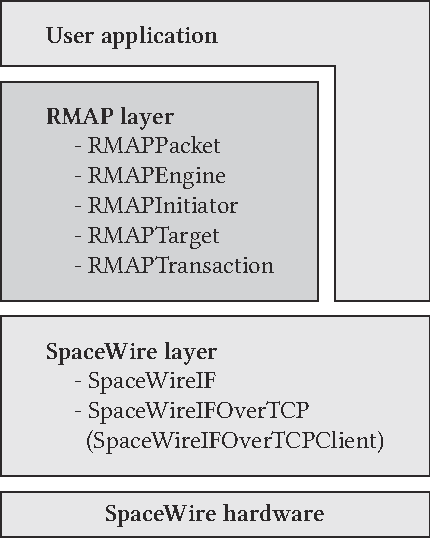
\includegraphics[width=7cm]{figures/SpaceWireRMAPLibrary/LibraryStructure.pdf}
\caption{An overall structure of SpaceWireRMAPLibrary.}\label{figure:LibraryStructure}
\end{figure}


\subsection{Folders}
SpaceWire RMAP Library consists of several folders as described below.
\begin{description}
\item[includes] contains header files of SpaceWire RMAP Library. In a user-application Makefile, add a path to this folder in the compiler flag.
\item[externalLibraries] contains CxxUtilities and XMLUtilities source trees for those who do not have their own installation of these libraries. The attached example Makefile uses these bundled libraries by default.
\item[exampleMakefile] contains an example Makefile for a user application which uses SpaceWire RMAP Library. Necessary compiler and linker flags are also described in the file.
\item[sources] contains free-gift programs built with SpaceWire RMAP Library, tutorial source code, and test codes.
\item[classic] contains obsolete (not maintained) SpaceWire RMAP Library v1 source tree.
\end{description}

\subsection{Files}
SpaceWire.hh and RMAP.hh are the top-level header files for SpaceWire and RMAP functionalities.
Load (\verb|#include|) them in a user application to use SpaceWire RMAP Library.
Tutorial given in \S\ref{section:tutorial} describes codes written in tutorial\_XXX.cc in the sources folder.
For details of main\_XXX files in the sources folder, see the following section. test\_XXX files contained in the sources folder are test codes written for checking implemented library functions. They are left as they are for Interested users' inspection.

\subsection{Free-gift programs}
In the sources folder, there are several main\_XXX.cc files.
These programs do very simple tasks using SpaceWire RMAP Library.
In ground experiments using SpaceWire and RMAP, these types of simple, standalone tasks are greatly powerful, and therefore, the developers bundled them as free gifts for users.

\begin{description}
\item[main\_RMAP\_calculateCRC] calculates CRC for an input byte sequence.
\item[main\_RMAP\_instructionToString] interprets single-byte RMAP instruction field value, and dumps its meaning.
\item[main\_RMAP\_interpretAsAnRMAPPacket] tries to interpret a provided byte sequence as an RMAP packet. When the interpretation is successful, resulting properties of the packet will be displayed as text.
\item[main\_RMAP\_readWriteRMAPTargetNode] performs simple RMAP read/write access to a specified RMAP target node.
\item[main\_RMAP\_replyStatusToString] converts a reply status value to string.
\end{description}



%%%%%%%%%%%%%%%%%%%%%%%%%%%%%%%%%%%%%%
%%%%%%%%%%%%%%%%%%%%%%%%%%%%%%%%%%%%%%
\section{Tutorial}\label{section:tutorial}
In the following subsections, a short walk-through of SpaceWire RMAP Library is described assuming that RMAP initiator is the most interested function for many users. Detailed usages and application specific topics related to SpaceWire and RMAP functions are presented in \S\ref{section:detailedUsages}.

For SpaceWire- and RMAP-layer tutorials, refer to tutorial source codes sources/tutorial\_SpaceWire.cc and sources/tutorial\_RMAP.cc. To compile these files, set the environmental variables (\S\ref{section:downloadAndSettings}), and then execute make in the SpaceWireRMAPLibrary/source/ folder.

\subsection{Use SpaceWire RMAP Library}
Include "SpaceWire.hh" and "RMAP.hh" for loading all necessary header files related to the SpaceWire and the RMAP layers.
Individual header files could be separately included for applications with limited usage of SpaceWire RMAP Library; e.g. a user application which only uses the RMAPPacket class, to include "RMAPPacket.hh" may be sufficient. Note that, practically, inclusion of "RMAP.hh" automatically includes "SpaceWire.hh".

Classes defined in SpaceWire RMAP Library are not enclosed with any namespace (i.e. declared at the root level).
However, classes of CxxUtilities are declared inside the namespace "CxxUtilities", and therefore, to use them, specify the full path of the class e.g. "CxxUtilities::Condition" or do "using namespace CxxUtilities;" in your source file.
Since Thread is a member of CxxUtilities, users may need to put "CxxUtilities::" when constructing a subclass of Thread (note "public CxxUtilities::Thread" not "public Thread").

\lstset{language=C++}
\begin{lstlisting}[label=source:sample_Thread_subclass]
class SubclassOfThread : public CxxUtilities::Thread {
public:
	void run(){
		... thread content ...
	}
};
\end{lstlisting}

\subsection{Summary of a virtual SpaceWire interface class}
List \ref{source:sample_SummaryOfSpaceWireIF} summarizes frequently used user-side interface provided by the SpaceWireIF class. See "SpaceWireIF.hh" for full details of each method. Implementation of virtual methods are given in SpaceWireIFXXX.cc, such as SpaceWireIFOverTCPClient.hh.

\lstset{language=C++,basicstyle=\ttfamily\scriptsize,tabsize=2,lineskip=0.5pt}
\begin{lstlisting}[label=source:sample_SummaryOfSpaceWireIF,caption=Summary of methods defined in SpaceWireIF.]
class SpaceWireIF {
public:
/* open/close */
	virtual void open() throw (SpaceWireIFException);
	virtual void close() throw (SpaceWireIFException);

/* send methods */
	virtual void
	send(uint8_t* data, size_t length, SpaceWireEOPMarker::EPPType eopType = SpaceWireEOPMarker::EOP) throw (SpaceWireIFException);
	virtual void
	send(std::vector<uint8_t>& data, SpaceWireEOPMarker::EPPType eopType = SpaceWireEOPMarker::EOP) throw (SpaceWireIFException);
	virtual void
	send(std::vector<uint8_t>* data, SpaceWireEOPMarker::EPPType eopType = SpaceWireEOPMarker::EOP) throw (SpaceWireIFException);

/* receive methods */
	//fast
	virtual std::vector<uint8_t>* receive() throw (SpaceWireIFException);
	//fast
	virtual void receive(std::vector<uint8_t>* buffer) throw (SpaceWireIFException);
	//slow; not recommended
	virtual void
	receive(uint8_t* buffer, SpaceWireEOPMarker::EPPType& eopType, size_t maxLength, size_t& length)	throw (SpaceWireIFException);

/* set receive timeout */
	virtual void setTimeoutDuration(double microsecond) throw (SpaceWireIFException);

/* emit timecode */
	virtual void emitTimecode(uint8_t timeIn, uint8_t controlFlagIn = 0x00) throw (SpaceWireIFException);

/* Action related to timecode */
	void addTimecodeAction(SpaceWireIFActionTimecodeScynchronizedAction* action);
	void registerTimecodeAction(SpaceWireIFActionTimecodeScynchronizedAction* action);
	void deleteTimecodeAction(SpaceWireIFActionTimecodeScynchronizedAction* action);
	void clearTimecodeSynchronizedActions();

/* Action related to link close event */
	void addSpaceWireIFCloseAction(SpaceWireIFActionCloseAction* spacewireIFCloseAction);
	void deleteSpaceWireIFCloseAction(SpaceWireIFActionCloseAction* spacewireIFCloseAction);
	void invokeSpaceWireIFCloseActions();

/* EOP/EEP related */
	bool isTerminatedWithEEP();
	bool isTerminatedWithEOP();
	void setReceivedPacketEOPMarkerType(int eopType);
	int getReceivedPacketEOPMarkerType();
	void eepShouldBeReportedAsAnException();
	void eepShouldNotBeReportedAsAnException();
};
\end{lstlisting}

\lstset{numbers=left,basicstyle=\ttfamily\footnotesize}
\lstset{language=C++,tabsize=4,lineskip=0.2pt}

\subsection{Opening/closing a SpaceWire interface}
SpaceWire RMAP Library provides a virtual interface for physical SpaceWire devices as defined in the super class SpaceWireIF.hh.
Classes named SpaceWireIFXXXX implements interface for real devices such as SpaceWire-to-GigabitEther
(i.e. SpaceWireIFOverTCPClient).

The super class defines a method name open() which opens a real SpaceWire interface device, and should be invoked when starting to use the device.
For example, in the case of SpaceWire-to-GigabitEther, use sentences below to construct an instance, and open the device.

Practically, SpaceWireIFOverTCPClient throws an exception when timeout occurs.
The example below tries to open the device (using the specified IP address), and the open() sentence is enclosed with a try-catch block to detect failure of opening a connection. The default port number is 10030, but this may not be always appropriate for different SpaceWire-to-GigabitEther. See user manual of your device. (for example, Shimafuji's SpaceWire-to-GigabitEther can accept 10031 as well for an additional SpaceWire-to-TCP/IP port)

\begin{lstlisting}[label=source:tutorial_SpaceWireIFOverTCP_open, caption=Sample code for opening SpaceWire-to-GigabitEther.]
/* Open the SpaceWire interface */
cout << "Opening SpaceWireIF...";
SpaceWireIF* spwif = new SpaceWireIFOverIPClient("192.168.1.100", 10030);
try {
	spwif->open();
} catch (...) {
	cerr << "Connection timed out." << endl;
	exit(-1);
}
cout << "done" << endl;

... user process using spwif ...

/* Close */
spwif->close();
\end{lstlisting}


\subsection{Sending/receiving SpaceWire packet}
Three types of send methods are available.
The only difference is a type of data container; C-array or std::vector.
Basic data type of SpaceWire RMAP Library is uint8\_t, and therefore containers should be uint8\_t* or std::vector<uint8\_t>.
Vectors can be passed as a reference or a pointer (the two ways result almost the same speed).

Parameters of the send methods are data (data content and length), and the end-of-packet (EOP) marker.
EOP markers is either of SpaceWireEOPMarker::EOP or SpaceWireEOPMarker::EEP.

When an exception occurs while sending a packet, the send method throws it to allow a user application to handle the situation.
The example below just dumps a reason of a thrown exception. Practically, users should think about re-trying to send the packet or  to notify the exception to higher layers.

\begin{lstlisting}[label=source:tutorial_SpaceWireIFOverTCP_send, caption=Sample code for sending packets.]
/* Send packet */
try {
	cout << "Send packet1" << endl;
	uint8_t packet1[] = { 0x0a, 0x0b, 0x0c, 0x0d };
	size_t length1 = 4;
	spwif->send(packet1, length1, SpaceWireIF::EOP);
	cout << "Send packet2" << endl;
	std::vector<uint8_t> packet2;
	packet2.push_back(0xe);
	packet2.push_back(0xf);
	packet2.push_back(1);
	packet2.push_back(2);
	packet2.push_back(3);
	spwif->send(packet2, SpaceWireIF::EOP);
} catch (SpaceWireIFException e) {
	cerr << "Exception when sending a packet." << endl;
	cerr << e.toString() << endl;
	exit(-1);
}
cout << "Send packet done" << endl;
\end{lstlisting}

List \ref{source:tutorial_SpaceWireIFOverTCP_settimeoutduration} sets a timeout duration for receive wait.
Note that implementation of timeout counter depends on SpaceWire interfaces, and precision may not be an order of microsecond.

\begin{lstlisting}[label=source:tutorial_SpaceWireIFOverTCP_settimeoutduration, caption=Sample code for setting a receive timeout duration.]
/* Set receive timeout */
spwif->setTimeoutDuration(1e6);//1sec timeout duration
\end{lstlisting}


List \ref{source:tutorial_SpaceWireIFOverTCP_receive} shows how to receive packets.
In the case of receive, std::vector<uint8\_t> is a default data container type since basically the size of a packet is unconstrained in SpaceWire (std::vector supports variable length data content, but C-array does not).
Two receive methods which interfaces with std::vector are available as used below. In the first example, a pointer to a newly constructed std::vector instance is returned when a packet is received. After processing the packet content, a user application should delete the instance (see \verb|delete packet3;|) although there is no explicit \verb|new| for this instance in this example (SpaceWireIF class internally constructs the instance). The second example is rather straightforward; an instance of std::vector<uint8\_t> is passed to the receive method.

\begin{lstlisting}[label=source:tutorial_SpaceWireIFOverTCP_receive, caption=Sample code for receiving packets.]
/* Receive packet */
cout << "Receive packet3" << endl;
try {
	std::vector<uint8_t>* packet3 = spwif->receive();
	cout << "Receive packet3 done (" << packet3->size() << "bytes)" << endl;
	//delete packet3 instance (it was newly constructed by SpaceWireIF internally,
	//and user should delete it to avoid memory leak.
	delete packet3;
} catch (SpaceWireIFException e) {
	if (e.getStatus() == SpaceWireIFException::Timeout) {
		cerr << "Receive timeout" << endl;
	} else {
		cerr << "Exception when receiving a packet." << endl;
		cerr << e.toString() << endl;
		exit(-1);
	}
}
cout << "Receive packet4" << endl;
try {
	std::vector<uint8_t>* packet4 = new std::vector<uint8_t>();
	spwif->receive(packet4);
	cout << "Receive packet4 done (" << packet4->size() << "bytes)" << endl;
	delete packet4;
} catch (SpaceWireIFException e) {
	if (e.getStatus() == SpaceWireIFException::Timeout) {
		cerr << "Receive timeout" << endl;
	} else {
		cerr << "Exception when receiving a packet." << endl;
		cerr << e.toString() << endl;
		exit(-1);
	}
}
\end{lstlisting}


\subsection{Emitting time codes}
In addition to the send/receive packet functions, SpaceWireIF is also able to emit time codes using the emitTimecode(uint8\_t timeIn, uint8\_t controlFlagIn = 0x00) method as shown in List \ref{source:tutorial_SpaceWireIFOverTCP_timecode}.
The timeIn parameter should contain a time code value from 0 to 63. The control flags are configurable to support possible future extensions of SpaceWire.

The example waits for 15.625 ms after sending one time code. Time-code value is incremented up to 63. The for loop consumes approximately 1 second to complete. Note that this is just an example, and time-code frequency is one of the most important parameter in a SpaceWire network. The frequency strongly depends on applications, and check if SpaceWire-to-GigabitEther achieves a required precision of emission frequency, and enough small jitter for your application. See SpaceWire-to-GigabitEther User Guide for details of jitters of time-code emission realized by SpaceWire-to-GigabitEther and SpaceWireIFOverTCPClient.

For periodic timecode emission, a thread class which has a similar code as List \ref{source:tutorial_SpaceWireIFOverTCP_timecode} in the run() method should be implemented, and started (i.e. call start()). See  excerpts in List \ref{source:tutorial_SpaceWireIFOverTCP_timecodePeriodic}, and tutorial\_SpaceWireLayer\_periodicTimecodeEmission.cc for full details.

\begin{lstlisting}[label=source:tutorial_SpaceWireIFOverTCP_timecode, caption=Sample code for emitting time codes.]
	/* Emit timecode */
	cout << "Emit timecode 64times" << endl;
	Condition c;
	try {
		for (uint8_t timecodeValue = 0; timecodeValue < 64; timecodeValue++) {
			cout << "Emitting timecode " << (uint32_t) timecodeValue << endl;
			spwif->emitTimecode(timecodeValue);
			c.wait(1.0 / 64.0); //wait 15.625ms
		}
	} catch (SpaceWireIFException e) {
		cerr << "Exception when receiving a packet." << endl;
		cerr << e.toString() << endl;
		exit(-1);
	}
\end{lstlisting}

\begin{lstlisting}[label=source:tutorial_SpaceWireIFOverTCP_timecodePeriodic, caption=Sample code for periodically emitting time codes.]
class TimecodeThread: public CxxUtilities::StoppableThread {
private:
	SpaceWireIF* spwif;

public:
	const static double TimecodeFrequency = 64; //Hz

public:
	TimecodeThread(SpaceWireIF* spwif) {
		this->spwif = spwif;
	}

public:
	void run() {
		uint8_t timecode = 0x00;
		while (!isStopped()) {
			try {
				spwif->emitTimecode(timecode);
			} catch (...) {
				using namespace std;
				cerr << "Timecode emission failed" << endl;
			}
			if (timecode == 63) {
				timecode = 0;
			} else {
				timecode++;
			}
			sleep(1 / TimecodeFrequency);
		}
	}
};
\end{lstlisting}

\subsection{Summary of RMAP-related classes}
For initiating RMAP transactions, user applications can use RMAPEngine and RMAPInitiator.
Information of an RMAP target node is handled being contained in an RMAPTargetNode instance.
For accepting RMAP commands and responding to them, subclasses of the RMAPTarget class can utilized with RMAPEngine.
Figure \ref{figure:SpaceWireRMAPStructure} shows a overall design of the SpaceWire and RMAP protocol stack used in SpaceWire RMAP Library.

\begin{figure}[htb]
\center
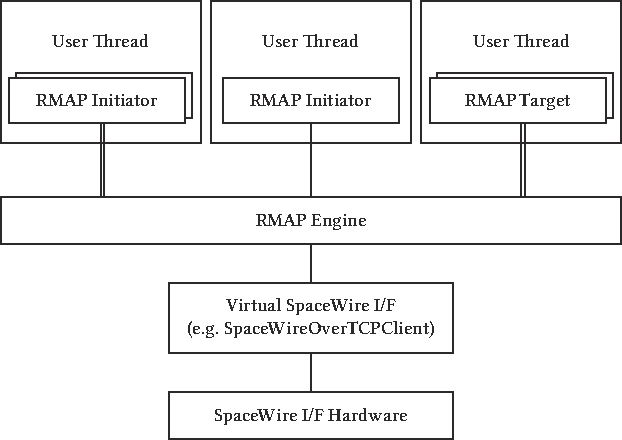
\includegraphics[width=8cm]{figures/SpaceWireRMAPLibrary/SpaceWireRMAPStructure.pdf}
\caption{SpaceWire and RMAP protocol stack in SpaceWire RMAP Library.}\label{figure:SpaceWireRMAPStructure}
\end{figure}

RMAPEngine works as a central engine of the RMAP functionality of a user application.
The tasks done by RMAPEngine includes 
issuing RMAP command packets, managing outstanding RMAP transactions, processing RMAP replies,
and responding to incoming RMAP commands.
RMAPInitiator bridges RMAPEngine and a user application providing easy-to-use read/write methods which implements RMAP read/write accesses.
RMAPTargetNode is used to pass necessary access information, such as target logical address, target SpaceWire address, and key of an accessed RMAP target node, to the read/write methods of RMAPInitiator.
Note that RMAPTargetNode corresponds to the RMAPDestination class defined in SpaceWire RMAP Library v1, but with many additional capabilities, particularly interface to an XML-line configuration file (see Appendix \ref{section:XMLLikeConfigurationFile}).

Lists \ref{source:summaryOfRMAPEngine}, \ref{source:summaryOfRMAPInitiator} and \ref{source:summaryOfRMAPTargetNode} summarizes a part of methods defined in the classes.
Less used methods are not shown, and therefore, refer RMAPEngine.hh and RMAPInitiator.hh for full details.

\begin{lstlisting}[label=source:summaryOfRMAPEngine, caption=RMAPEngine methods (excerpts).]
class RMAPEngine: public CxxUtilities::Thread {
public:

/* constructor */
	RMAPEngine(SpaceWireIF* spwif);

/* start/stop */
	virtual void start();
	void stop();
	bool isStopped();
	bool isStarted();

/* methods used by RMAPInitiator */
	void initiateTransaction(RMAPTransaction* transaction) throw (RMAPEngineException);
	void cancelTransaction(RMAPTransaction* transaction) throw (RMAPEngineException);

/* raw packet send method which even can be used while RMAPEngine is running */
	void sendPacket(std::vector<uint8_t>* bytes);

/* methods used when a user application implements an RMAPTarget */
	void addRMAPTarget(RMAPTarget* rmapTarget);
	void removeRMAPTarget(RMAPTarget* rmapTarget);

/* accessor for a SpaceWireIF instance */
	void setSpaceWireIF(SpaceWireIF* spwif);
	SpaceWireIF* getSpaceWireIF();

/* actions invoked when RMAPEngine is stopped (automatically or manually) */
	void addRMAPEngineStoppedAction(RMAPEngineStoppedAction* rmapEngineStoppedAction);
	void removeRMAPEngineStoppedAction(RMAPEngineStoppedAction* rmapEngineStoppedAction);
	CxxUtilities::Actions* getRMAPEngineStoppedActions();
};
\end{lstlisting}

\begin{lstlisting}[label=source:summaryOfRMAPInitiator, caption=RMAPInitiator methods (excerpts).]
class RMAPInitiator {
public:
/* constructor */
	RMAPInitiator(RMAPEngine *rmapEngine);

/* RMAP Read methods */
	/* fast */
	void read(RMAPTargetNode* rmapTargetNode, uint32_t memoryAddress,
			uint32_t length, uint8_t *buffer, double timeoutDuration = DefaultTimeoutDuration)
			throw (RMAPEngineException, RMAPInitiatorException, RMAPReplyException);

	/* easy to use, but somewhat slow due to data copy. */
	/* this methods returns a pointer to a newly constructed std::vector instance */
	std::vector<uint8_t>* readConstructingNewVecotrBuffer(std::string targetNodeID,
			std::string memoryObjectID, double timeoutDuration = DefaultTimeoutDuration)
			throw (RMAPEngineException, RMAPInitiatorException, RMAPReplyException);

	/* convenient, but somewhat slow due to RMAPTargetNode DB and  RMAPMemoryObject DB search */
	void read(std::string targetNodeID, std::string memoryObjectID, uint8_t* buffer,
			double timeoutDuration = DefaultTimeoutDuration)
			throw (RMAPEngineException, RMAPInitiatorException, RMAPReplyException);

	/* convenient, but somewhat slow due to RMAPTargetNode DB search */
	void read(std::string targetNodeID, uint32_t memoryAddress, uint32_t length,
			uint8_t* buffer, double timeoutDuration = DefaultTimeoutDuration)
			throw (RMAPEngineException, RMAPInitiatorException, RMAPReplyException);

	/* convenient, but somewhat slow due to RMAPMemoryObject DB search */
	void read(RMAPTargetNode* rmapTargetNode, std::string memoryObjectID,
			uint8_t *buffer, double timeoutDuration = DefaultTimeoutDuration)
			throw (RMAPEngineException, RMAPInitiatorException, RMAPReplyException);

/* RMAP Write methods */
	/* fast */
	void write(RMAPTargetNode *rmapTargetNode, uint32_t memoryAddress,
			uint8_t *data, uint32_t length, double timeoutDuration = DefaultTimeoutDuration)
			throw (RMAPEngineException, RMAPInitiatorException, RMAPReplyException);

	/* convenient, but somewhat slow due to RMAPTargetNode DB and  RMAPMemoryObject DB search */
	void write(std::string targetNodeID, std::string memoryObjectID, uint8_t* data,
			double timeoutDuration = DefaultTimeoutDuration)
			throw (RMAPEngineException, RMAPInitiatorException, RMAPReplyException);
	
	/* convenient, but somewhat slow due to RMAPTargetNode DB search */
	void write(std::string targetNodeID, uint32_t memoryAddress, uint8_t *data,
			uint32_t length, double timeoutDuration = DefaultTimeoutDuration)
			throw (RMAPEngineException, RMAPInitiatorException, RMAPReplyException);

	/* convenient, but somewhat slow due to RMAPMemoryObject DB search */
	void write(RMAPTargetNode *rmapTargetNode, std::string memoryObjectID,
			uint8_t* data, double timeoutDuration = DefaultTimeoutDuration)
			throw (RMAPEngineException, RMAPInitiatorException, RMAPReplyException);
	

/* set/get logical address of this RMAPInitiator */
	void setInitiatorLogicalAddress(uint8_t initiatorLogicalAddress);
	uint8_t getInitiatorLogicalAddress();

/* accessor for other RMAP options */
	void setReplyMode(bool replyMode);
	void unsetReplyMode();
	bool isReplyModeSet();

	void setIncrementMode(bool incrementMode);
	void unsetIncrementMode();
	bool isIncrementModeSet();

	void setVerifyMode(bool verifyMode);
	void unsetVerifyMode();
	bool isVerifyModeSet();

	void setTransactionID(uint16_t transactionID);
	void unsetTransactionID();
	uint16_t getTransactionID();
	bool isTransactionIDSet();

/* accessor for raw packet pointer */
	RMAPPacket* getCommandPacketPointer();
	RMAPPacket* getReplyPacketPointer();

/* interface for RMAPTargetNodeDB */
	void setRMAPTargetNodeDB(RMAPTargetNodeDB* targetNodeDB);
	RMAPTargetNodeDB* getRMAPTargetNodeDB();
};
\end{lstlisting}


\begin{lstlisting}[label=source:summaryOfRMAPTargetNode, caption=RMAPTargetNode methods (excerpts).]
class RMAPTargetNode: public RMAPNode {
public:
/* constructor */
	RMAPTargetNode();

/* interfaces to XML-like configuration file */
	static std::vector<RMAPTargetNode*> constructFromXMLFile(std::string filename)
		throw (XMLLoader::XMLLoaderException, RMAPTargetNodeException, RMAPMemoryObjectException);

	static std::vector<RMAPTargetNode*> constructFromXMLFile(XMLNode* topNode)
		throw (XMLLoader::XMLLoaderException, RMAPTargetNodeException, RMAPMemoryObjectException);

	static RMAPTargetNode* constructFromXMLNode(XMLNode* node)
		throw (XMLLoader::XMLLoaderException, RMAPTargetNodeException, RMAPMemoryObjectException);

/* accessor for options */
	uint8_t getDefaultKey();
	void setDefaultKey(uint8_t defaultKey);

	std::vector<uint8_t> getReplyAddress();
	void setReplyAddress(std::vector<uint8_t>& replyAddress);

	uint8_t getTargetLogicalAddress();
	void setTargetLogicalAddress(uint8_t targetLogicalAddress);

	std::vector<uint8_t> getTargetSpaceWireAddress();
	void setTargetSpaceWireAddress(std::vector<uint8_t>& targetSpaceWireAddress);

	void setInitiatorLogicalAddress(uint8_t initiatorLogicalAddress);
	void unsetInitiatorLogicalAddress();
	bool isInitiatorLogicalAddressSet();
	uint8_t getInitiatorLogicalAddress();

/* dealing with memory objects available on an RMAPTargetNode */
	void addMemoryObject(RMAPMemoryObject* memoryObject);
	std::map<std::string, RMAPMemoryObject*>* getMemoryObjects();

/* accessor for registered memory objects */
	RMAPMemoryObject* getMemoryObject(std::string memoryObjectID)
		throw (RMAPTargetNodeException);
	RMAPMemoryObject* findMemoryObject(std::string memoryObjectID)
		throw (RMAPTargetNodeException);

/* converts an instance to string or XML string */
	std::string toString(int nTabs = 0);
	std::string toXMLString(int nTabs = 0);
};
\end{lstlisting}



\subsection{RMAP read/write using RMAPEngine and RMAPInitiator}
RMAPInitiator works with RMAPEngine, and therefore, an RMAPEngine instance should be first constructed, and started to work as List \ref{source:tutorial_RMAPLayer_constructInstances} presents.
RMAPEngine is a subclass of CxxUtilities::Thread, and has start() method to fork a new thread which waits for incoming packets in the background of the main thread (usually, a user application thread). Since RMAPEngine uses SpaceWireIF, its constructor accepts a pointer to a SpaceWireIF instance. An RMAPInitiator instance should be constructed with a pointer to the RMAPEngine instance. An initiator logical address can be set (the example below just sets the default value 0xFE, but any number 0x20-0xFD could be specified).

Note that multiple RMAPInitiator instances can be constructed, and tied to one RMAPEngine. This allows concurrent multiple transaction using a single SpaceWire interface. There is virtually no limit on the number of RMAPInitiator instances registered to one RMAPEngine. When a user application communicates with many RMAP targets, it is basically strongly recommended to create multiple RMAPInitiator instances and perform read/write transactions concurrently so as to improve bandwidth usage (i.e. for higher data transfer speed).

\begin{lstlisting}[label=source:tutorial_RMAPLayer_constructInstances, caption=Sample code for constructing RMAPEngine/RMAPInitiator.]
/* Construct and start RMAP Engine */
RMAPEngine* rmapEngine = new RMAPEngine(spwif);
rmapEngine->start();

/* Construct an RMAP Initiator instance */
RMAPInitiator* rmapInitiator = new RMAPInitiator(rmapEngine);
rmapInitiator->setInitiatorLogicalAddress(0xFE);
\end{lstlisting}


List \ref{source:tutorial_RMAPLayer_readWriteCase1} executes RMAP read/write using a manually constructed RMAPTargetNode instance. Read buffers can be either of C-array and std::vector<uint8\_t>. Write data are expected to be passed using C-array (std::vector<uint8\_t>::begin() could be used as well). When performing read/write accesses, time-out duration can be passed as a parameter to avoid infinite wait for a reply packet (when target node information is incorrect or an RMAP target is not working, a reply packet may not be received by RMAPEngine, and therefore, generally, RMAPInitiator should terminate wait at a certain point).

RMAP options, such as reply mode, verification mode, address increment mode, and so on, can be set via RMAPInitiator methods (see List \ref{source:summaryOfRMAPInitiator}). Default values of these options can be found (even changed) in RMAPProtocol.hh.

\begin{lstlisting}[label=source:tutorial_RMAPLayer_readWriteCase1, caption=Sample code for performing RMAP read/write using a manually constructed RMAPTargetNode instance.]
/////////////////////////////////////////////////////////////////////////////////////
/* Example 1 */
/* Manually sets RMAPTargetNode information */
cout << "Example 1" << endl;

RMAPTargetNode rmapTargetNode1;
rmapTargetNode1.setTargetLogicalAddress(0xfe);
rmapTargetNode1.setDefaultKey(0x20);
std::vector<uint8_t> targetSpaceWireAddress;
targetSpaceWireAddress.push_back(0x01);
targetSpaceWireAddress.push_back(0x0a);
targetSpaceWireAddress.push_back(0x05);
rmapTargetNode1.setTargetSpaceWireAddress(targetSpaceWireAddress);
std::vector<uint8_t> replyAddress;
replyAddress.push_back(0x08);
replyAddress.push_back(0x03);
replyAddress.push_back(0x0f);
rmapTargetNode1.setReplyAddress(replyAddress);
cout << rmapTargetNode1.toString() << endl;
/* RMAP Read/Write with address/length */
try {
	//case 1-1 : using C-array as a read buffer
	uint32_t readLength = 1024;
	uint8_t* readData = new uint8_t[(size_t) readLength];
	uint32_t readAddress = 0xFF801100;
	rmapInitiator->
		read(rmapTargetNode1, readAddress, readLength, readData, readTimeoutDuration);
	//case 1-2 : using std::vector<uint8_t> as a read buffer
	std::vector<uint8_t> readDataVector;
	rmapInitiator->
		read(rmapTargetNode1, readAddress, readLength,
			(uint8_t*)readDataVector.begin(), readTimeoutDuration);

	//case 1-3 : write using C-array write data
	uint32_t writeAddress = 0xFF803800;
	uint32_t writeLength = 4;
	uint8_t* writeData = new uint8_t[writeLength];
	writeData[0] = 0xAB;
	writeData[1] = 0xCD;
	writeData[2] = 0x12;
	writeData[3] = 0x34;
	rmapInitiator->
		write(rmapTargetNode1, writeAddress, writeData, writeLength, writeTimeoutDuration);
		
	delete readData;
	delete writeData;
	delete rmapTargetNode1;
	
	cout << "RMAP Read/Write Example1 done" << endl;
	
} catch (RMAPInitiatorException e) {
	cerr << "RMAPInitiatorException " << e.toString() << endl;
	cerr << "Continue to next example" << endl;
} catch (RMAPReplyException e) {
	cerr << "RMAPReplyException " << e.toString() << endl;
	cerr << "Continue to next example" << endl;
} catch (RMAPEngineException e) {
	cerr << "RMAPEngineException " << e.toString() << endl;
	cerr << "Continue to next example" << endl;
} catch (...) {
	cerr << "Unkown error" << endl;
	exit(-1);
}
/////////////////////////////////////////////////////////////////////////////////////
\end{lstlisting}


\subsection{RMAP read/write specifying IDs of RMAP target nodes (using RMAPTargetNodeDB)}
RMAPTargetNode instances can be constructed following information described in an XML-like configuration file.
RMAPTargetNodeDB is a collection of RMAPTargetNode instances, and the class provides an easy-to-use constructor "RMAPTargetNodeDB:: RMAPTargetNodeDB( std::string filename);" which loads all the RMAPTargetNode defined in the file. List \ref{source:tutorial_RMAPLayer_readWriteCase2} shows how to load a configuration file.
Note that RMAPTargetNode information in the XML file can contain information of memory objects on an RMAP target node such as identifier, memory address, length, and access mode (see Appendix \ref{section:XMLLikeConfigurationFile}).

An RMAPInitiator instance accepts an instance of RMAPTargetNodeDB as a data base of RMAP target nodes, and read/write methods are invoked with identifiers of an RMAPTargetNode and a memory object on it as used in List \ref{source:tutorial_RMAPLayer_readWriteCase2}. Since there should occur database lookups (for RMAPTargetNode and RMAPMemoryObject), these methods are slightly slower than the ones explained in the previous section which uses RMAPTargetNode*, memory address, and length directly. However, these ID-specifying methods are still very useful because of higher reconfigurability, and modularity of the source code; even when a network configuration and register mapping are changed, it is not necessary to modify source codes, but a configuration file can be easily updated to take into account those changes.

When specified RMAPTargetNode ID or memory object ID is not found in RMAPTargetNodeDB, RMAPInitiator will throw
 RMAPInitiatorException with status of RMAPInitiatorException::NoSuchRMAPTargetNode or RMAPInitiatorException::NoSuchRMAPMemoryObject.

\begin{lstlisting}[label=source:tutorial_RMAPLayer_readWriteCase2, caption=Sample code for performing RMAP read/write using an RMAPTargetNode instance contained in an RMAPTargetNodeDB constructed from an XML-like configuration file.]
/////////////////////////////////////////////////////////////////////////////////////
/* Example 2 */
/* Use RMAPTargetNodes constructed from an XML-like configuration file. */
cout << "Example 2" << endl;
if (argc < 2) {
	cerr << "Example2 requires an XML-like configuration file." << endl;
	exit(-1);
}

//check file existence
if (!CxxUtilities::File::exists(argv[1])) {
	cerr << "File " << argv[1] << " does not exist." << endl;
	exit(-1);
}

//construct RMAPTargetNodes from the XML file
std::string filename(argv[1]);
cout << "Constructing RMAPTargetNodes from " << filename << endl;
RMAPTargetNodeDB* rmapTargetNodeDB;
try {
	rmapTargetNodeDB = new RMAPTargetNodeDB(filename);
} catch (RMAPTargetNodeDBException e) {
	cerr << "An exception thrown while loading the XML file " << filename << endl;
	cerr << e.toString() << endl;
	exit(-1);
}

//check the number of entries
if (rmapTargetNodeDB->getSize() == 0) {
	cerr << "No RMAPTargetNode instance was constructed..." << endl;
	exit(-1);
}

//set the db to RMAPInitiator
rmapInitiator->setRMAPTargetNodeDB(rmapTargetNodeDB);

/* RMAP Read/Write with address/length */
try {
	//case 1-1 : read using C-array as a read buffer
	uint32_t readLength = 2;
	uint8_t* readData = new uint8_t[(size_t) readLength];
	rmapInitiator->
		read("SpaceWireDigitalIOBoard", "LEDRegister", readData, readTimeoutDuration);

	//case 1-2 : read using std::vector<uint8_t> as a read buffer
	std::vector<uint8_t> readDataVector(readLength);
	rmapInitiator->
		read("SpaceWireDigitalIOBoard", "LEDRegister", &(readDataVector.at(0)), readTimeoutDuration);

	//case 1-3 : write using C-array write data
	uint32_t writeLength = 2;
	uint8_t* writeData = new uint8_t[writeLength];
	writeData[0] = 0xFF;
	writeData[1] = 0xFF;
	rmapInitiator->
		write("SpaceWireDigitalIOBoard", "LEDRegister", writeData, writeTimeoutDuration);

	delete readData;
	delete writeData;

	cout << "RMAP Read/Write Example2 done" << endl;

} catch (RMAPInitiatorException e) {
	cerr << "RMAPInitiatorException " << e.toString() << endl;
	cerr << "Continue to next example" << endl;
} catch (RMAPReplyException e) {
	cerr << "RMAPReplyException " << e.toString() << endl;
	cerr << "Continue to next example" << endl;
} catch (RMAPEngineException e) {
	cerr << "RMAPEngineException " << e.toString() << endl;
	cerr << "Continue to next example" << endl;
} catch (...) {
	cerr << "Unkown error" << endl;
	exit(-1);
}
/////////////////////////////////////////////////////////////////////////////////////
\end{lstlisting}


\subsection{RMAP Packet creation/interpretation}
The RMAPPacket class provides integrated functionalities of RMAP packet creation/interpretation.
List \ref{} summarizes representative methods available in RMAPPacket.

\begin{lstlisting}[label=source:tutorial_RMAPPacket_example1, caption=Sample code for manually constructing an RMAP packet.]
class RMAPPacket {
	bool 	getDataCRCIsChecked ();
	bool 	getHeaderCRCIsChecked ();
	void 	setDataCRCIsChecked (bool dataCRCIsChecked);
	void 	setHeaderCRCIsChecked (bool headerCRCIsChecked);
	void 	constructHeader ();
	void 	calculateDataCRC ();
	void 	constructPacket ();
	std::vector< uint8_t > 	getPacket ();
	std::vector< uint8_t > * 	getPacketBufferPointer ();
	void 	interpretAsAnRMAPPacket (uint8_t *packet, size_t length) throw (RMAPPacketException);
	void 	interpretAsAnRMAPPacket (std::vector< uint8_t > &data) throw (RMAPPacketException);
	void 	interpretAsAnRMAPPacket (std::vector< uint8_t > *data) throw (RMAPPacketException);
	void 	setRMAPTargetInformation (RMAPTargetNode *rmapTargetNode);
	void 	setRMAPTargetInformation (RMAPTargetNode &rmapTargetNode);
	bool 	isCommand ();
	void 	setCommand ();
	bool 	isReply ();
	void 	setReply ();
	bool 	isWrite ();
	void 	setWrite ();
	bool 	isRead ();
	void 	setRead ();
	bool 	isVerifyFlagSet ();
	void 	setVerifyFlag ();
	void 	unsetVerifyFlag ();
	void 	setVerifyMode ();
	void 	setNoVerifyMode ();
	bool 	isReplyFlagSet ();
	void 	setReplyFlag ();
	void 	unsetReplyFlag ();
	void 	setReplyMode ();
	void 	setNoReplyMode ();
	bool 	isIncrementFlagSet ();
	void 	setIncrementFlag ();
	void 	unsetIncrementFlag ();
	void 	setIncrementMode ();
	void 	setNoIncrementMode ();
	uint8_t 	getReplyPathAddressLength ();
	void 	setReplyPathAddressLength (uint8_t pathAddressLength);
	uint32_t 	getAddress ();
	bool 	hasData ();
	std::vector< uint8_t > 	getData ();
	void 	getData (uint8_t *buffer, size_t maxLength) throw (RMAPPacketException);
	void 	getData (std::vector< uint8_t > &buffer);
	void 	getData (std::vector< uint8_t > *buffer);
	std::vector< uint8_t > * 	getDataBuffer ();
	uint8_t 	getDataCRC ();
	uint32_t 	getDataLength ();
	uint32_t 	getLength ();
	uint8_t 	getExtendedAddress ();
	uint8_t 	getHeaderCRC ();
	uint8_t 	getInitiatorLogicalAddress ();
	uint8_t 	getInstruction ();
	uint8_t 	getKey ();
	uint8_t 	getProtocolID ();
	std::vector< uint8_t > 	getReplyAddress ();
	uint8_t 	getTargetLogicalAddress ();
	std::vector< uint8_t > 	getTargetSpaceWireAddress ();
	uint16_t 	getTransactionID ();
	void 	setAddress (uint32_t address);
	void 	setData (std::vector< uint8_t > &data);
	void 	setData (uint8_t *data, size_t length);
	void 	setDataCRC (uint8_t dataCRC);
	void 	setDataLength (uint32_t dataLength);
	void 	setLength (uint32_t dataLength);
	void 	setExtendedAddress (uint8_t extendedAddress);
	void 	setHeaderCRC (uint8_t headerCRC);
	void 	setInitiatorLogicalAddress (uint8_t initiatorLogicalAddress);
	void 	setInstruction (uint8_t instruction);
	void 	setKey (uint8_t key);
	void 	setProtocolID (uint8_t protocolID);
	void 	setReplyAddress (std::vector< uint8_t > replyAddress, bool automaticallySetPathAddressLengthToInstructionField=true);
	void 	setTargetLogicalAddress (uint8_t targetLogicalAddress);
	void 	setTargetSpaceWireAddress (std::vector< uint8_t > targetSpaceWireAddress);
	void 	setTransactionID (uint16_t transactionID);
	uint8_t 	getStatus ();
	void 	setStatus (uint8_t status);
	uint32_t 	getHeaderCRCMode ();
	void 	setHeaderCRCMode (uint32_t headerCRCMode);
	uint32_t 	getDataCRCMode ();
	void 	setDataCRCMode (uint32_t dataCRCMode);
	void 	addData (uint8_t oneByte);
	void 	clearData ();
	void 	addData (std::vector< uint8_t > array);
	std::string 	toString ();
	std::string 	toXMLString ();
	void 	toStringInstructionField (std::stringstream &ss);
	std::string 	toXMLStringCommandPacket (int nTabs=0);
	std::string 	toXMLStringReplyPacket (int nTabs=0);
};
\end{lstlisting}

List \ref{source:tutorial_RMAPPacket_example1} presents an example of manual packet creation using RMAPPacket excerpted from tutorial \_RMAPPacket \_creationInterpretation.cc.
After setting many options, RMAPPacket::constructPacket() which compiles header, calculates CRCs, and concatenates the header and the data part. Resulting byte sequence can be obtained by calling RMAPPacket:: getPacketBufferPointer() as a std::vector pointer.
To display an RMAPPacket, RMAPPacket::toString() or toXMLString() can be utilized.
An execution result is shown in List \ref{source:tutorial_RMAPPacket_example1result}.

\begin{lstlisting}[label=source:tutorial_RMAPPacket_example1, caption=Sample code for manually constructing an RMAP packet.]
//Example1 : Manually construct an RMAP packet
vector<uint8_t> targetSpaceWireAddress;
targetSpaceWireAddress.push_back(3);
targetSpaceWireAddress.push_back(10);
targetSpaceWireAddress.push_back(21);
vector<uint8_t> replyAddress;
replyAddress.push_back(5);
replyAddress.push_back(3);
uint32_t dataLength = 0x31;
RMAPPacket rmapPacket1;
rmapPacket1.setTargetSpaceWireAddress(targetSpaceWireAddress);
rmapPacket1.setReplyAddress(replyAddress);
rmapPacket1.setWrite();
rmapPacket1.setCommand();
rmapPacket1.setIncrementMode();
rmapPacket1.setNoVerifyMode();
rmapPacket1.setExtendedAddress(0x00);
rmapPacket1.setAddress(0xff803800);
rmapPacket1.setDataLength(dataLength);
for (size_t i = 0; i < dataLength; i++) {
	rmapPacket1.addData((uint8_t) i);
}
rmapPacket1.constructPacket();
cout << "RMAPPacket1" << endl;
SpaceWireUtilities::dumpPacket(rmapPacket1.getPacketBufferPointer());
cout << "----------------------------" << endl;
rmapPacket1.setHeaderCRCMode(RMAPPacket::AutoCRC);
rmapPacket1.constructHeader();
cout << rmapPacket1.toString() << endl;
cout << rmapPacket1.toXMLString() << endl;
cout << endl;
\end{lstlisting}

\begin{lstlisting}[language=bash,label=source:tutorial_RMAPPacket_example1result, caption=Result of Example1 of tutorial\_RMAPPacket\_creationInterpretation.cc.]
--------- Target SpaceWire Address ---------
0x03 0x0a 0x15 
--------- RMAP Header Part ---------
Initiator Logical Address : 0x00
Target Logic. Address     : 0xfe
Protocol ID               : 0x01
Instruction               : 0x65
 ------------------------------
 |Reserved    : 0
 |Packet Type : 1 (Command)
 |Write/Read  : 1 (Write)
 |Verify Mode : 0 (No Verify)
 |Reply Mode  : 0 (No Reply)
 |Increment   : 1 (Increment)
 |R.A.L.      : 1
 |(R.A.L. = Reply Address Length)
 ------------------------------
Key                       : 0x20
Reply Address             : 0x05 0x03 
Transaction Identifier    : 0x0000
Extended Address          : 0x00
Address                   : 0xff803800
Data Length (bytes)       : 0x000031 (49dec)
Header CRC                : 0x8b
---------  RMAP Data Part  ---------
[data size = 49bytes]
0x00 0x01 0x02 0x03 0x04 0x05 0x06 0x07 0x08 0x09 0x0a 0x0b 0x0c 0x0d 0x0e 0x0f 
0x10 0x11 0x12 0x13 0x14 0x15 0x16 0x17 0x18 0x19 0x1a 0x1b 0x1c 0x1d 0x1e 0x1f 
0x20 0x21 0x22 0x23 0x24 0x25 0x26 0x27 0x28 0x29 0x2a 0x2b 0x2c 0x2d 0x2e 0x2f 
0x30 
Data CRC                  : 81

Total data (bytes)        : 73
\end{lstlisting}


List \ref{source:tutorial_RMAPPacket_example2} interprets an example byte sequence as an RMAP packet.
If RMAPPacket:: interpretAsAnRMAPPacket( uint8\_t *packet, size\_t length) returns with no exception,
the byte sequence is a valid RMAP packet, and interpreted properties are accessible from the RMAPPacket instance.
When an exception is thrown, inspect the status and try to disable CRC checks (if RMAPPacketException::InvalidHeaderCRC or RMAPPacketException::InvalidDataCRC is thrown). This can be done via RMAPPacket:: setHeaderCRCIsChecked( bool) or RMAPPacket:: setDataCRCIsChecked( bool). By default, validities of header and data CRCs are checked, and an exception will be thrown when either or both of them are invalid. List \ref{source:tutorial_RMAPPacket_example2result} shows an execution result of List \ref{source:tutorial_RMAPPacket_example2}.

\begin{lstlisting}[label=source:tutorial_RMAPPacket_example2, caption=Sample code for manually interpreting an RMAP packet.]
//Example2 : Interpret a byte sequence as an RMAP packet
RMAPPacket rmapPacket2;
uint8_t bytes[] =
		{ 0x07, 0x0B, 0x06, 0x04, 0xFE, 0x01, 0x4F, 0x91,
			00, 00, 00, 00, 00, 00, 00, 0x02, 0x0C, 0x0A,
			0x04, 0x06, 0xFE, 0xAD, 0xDF, 0x00, 0xFF, 0x80, 0x11, 0x00,
			0x00, 0x00, 0x10, 0x2A };
try {
	rmapPacket2.interpretAsAnRMAPPacket(bytes, sizeof(bytes));
} catch (RMAPPacketException e) {
	cerr << "RMAPPacketException " << e.toString() << endl;
	exit(-1);
}
cout << "RMAPPacket2" << endl;
SpaceWireUtilities::dumpPacket(rmapPacket2.getPacketBufferPointer());
cout << "----------------------------" << endl;
rmapPacket2.setHeaderCRCMode(RMAPPacket::AutoCRC);
rmapPacket2.constructHeader();
cout << rmapPacket2.toString() << endl;
cout << rmapPacket2.toXMLString() << endl;
\end{lstlisting}

\begin{lstlisting}[label=source:tutorial_RMAPPacket_example2result, caption=Result of Example2 of tutorial\_RMAPPacket\_creationInterpretation.cc.]
--------- Target SpaceWire Address ---------
0x07 0x0b 0x06 0x04 
--------- RMAP Header Part ---------
Initiator Logical Address : 0xfe
Target Logic. Address     : 0xfe
Protocol ID               : 0x01
Instruction               : 0x4f
 ------------------------------
 |Reserved    : 0
 |Packet Type : 1 (Command)
 |Write/Read  : 0 (Read)
 |Verify Mode : 0 (No Verify)
 |Reply Mode  : 1 (Reply)
 |Increment   : 1 (Increment)
 |R.A.L.      : 3
 |(R.A.L. = Reply Address Length)
 ------------------------------
Key                       : 0x91
Reply Address             : 0x00 0x00 0x00 0x00 0x00 0x00 0x00 0x02 0x0c 0x0a 0x04 0x06 
Transaction Identifier    : 0xaddf
Extended Address          : 0x00
Address                   : 0xff801100
Data Length (bytes)       : 0x000010 (16dec)
Header CRC                : 0x2a
---------  RMAP Data Part  ---------
--- none ---

Total data (bytes)        : 32


<RMAPPacket>
	<ProtocolID>0x01</ProtocolID>
	<InitiatorLogicalAddress>0xfe</InitiatorLogicalAddress>
	<TargetLogicalAddress>0xfe</TargetLogicalAddress>
	<TargetSpaceWireAddress>0x07  0x0b  0x06  0x04</TargetSpaceWireAddress>
	<ReplyAddress>0x00  0x00  0x00  0x00  0x00  0x00  0x00  0x02  0x0c  0x0a  0x04  0x06</ReplyAddress>
	<Instruction>0x4f</Instruction>
	<Key>0x91</Key>
	<TransactionIdentifier>0xaddf</TransactionIdentifier>
	<ExtendedAddress>0x00</ExtendedAddress>
	<Address>0xff801100</Address>
	<Length>0x10</Length>
	<HeaderCRC>Auto</HeaderCRC>
	<!-- HeaderCRC = 0x2a (as long as the header is intact) -->
</RMAPPacket>
\end{lstlisting}


\subsection{Multithread and inter-thread communication}
%start()���ĂԂƁA�X���b�h����������邱��
%stoppable thread

%condition
%mutex
%timeout

%%%%%%%%%%%%%%%%%%%%%%%%%%%%%%%%%%%%%%
%%%%%%%%%%%%%%%%%%%%%%%%%%%%%%%%%%%%%%
\section{Detailed usages of the SpaceWire and the RMAP layers}\label{section:detailedUsages}
This section, and the following RMAP section, will be updated upon requests from users. If you have any question or comment on a specific function of SpaceWire RMAP Library. 

\subsection{Handling an interface-close event}
A SpaceWire interface might be suddenly closed outside the user control due to several reasons (e.g. disconnection of a TCP/IP socket in SpaceWireIFOverTCPClient). This kind of event should be reported to a user application layer so that it can handle the situation, and not to use the same (closed) interface any more (i.e. not to send/receive packets).

SpaceWireIF uses a call-back framework for notifying such an event to a user application.
Relevant class and methods include SpaceWireIFActionCloseAction, and
SpaceWireIF:: addSpaceWireIFCloseAction( SpaceWireIFActionCloseAction* spacewireIFCloseAction).
Instances of subclasses of SpaceWireIFActionCloseAction can be registered to a SpaceWireIF instance,
and these action instances, more precisely its SpaceWireIFActionCloseAction:: doAction (SpaceWireIF*) method, are invoked when SpaceWireIF::close() is called by a user application or by other thread running in the background.

SpaceWire RMAP GUI available from the open-source SpaceWire project uses this call-back mechanism to know SpaceWireIF-close events, and to stop data transfer. See SpaceWire RMAP GUI source code, particularly SpaceWireViewController.h, for practical example. List \ref{source:sampleSubclassOfSpaceWireIFActionCloseAction} presents an example of a subclass of SpaceWireIFActionCloseAction defined in SpaceWire RMAP GUI.

\begin{lstlisting}[label=source:sampleSubclassOfSpaceWireIFActionCloseAction, caption=An example of a subclass of SpaceWireIFActionCloseAction.]
class SpaceWireViewContollerCloseActionStopContinuousReceive : public SpaceWireIFActionCloseAction {
private:
        id spacewireViewController;
public:
        SpaceWireViewContollerCloseActionStopContinuousReceive(id spacewireViewController){
                this->spacewireViewController=spacewireViewController;
        }
        
public:
        void doAction(SpaceWireIF* spacewireIF){
                [spacewireViewController stopContinuousPacketReceive];
                [spacewireViewController stopPeriodicTimecodeEmission];
        }
};
\end{lstlisting}


\subsection{Timecode-synchronized action}
Timecode-synchronized actions are also implemented as a call-back to registered instances of the SpaceWireIFAction TimecodeScynchronizedAction class (see SpaceWireIF.hh) as was described in the previous section for interface-close event actions.

Users can implement subclasses of SpaceWireIFAction TimecodeScynchronizedAction, and the doAction( unsigned char timecodeValue) method is invoked, via SpaceWireIF::invokeSpaceWireIFCloseActions(), every time when a timecode is received. Filtering of timecode values should be done in the method by users. As presented in List \ref{source:invokeSpaceWireIFCloseActions}, registered timecode-synchronized actions are invoked sequentially, and therefore, time-consuming processes should be avoided in the doAction( unsigned char timecodeValue) method (if time-consuming process should be done, start another thread in the action, and yield main process to the following action instances).

\begin{lstlisting}[label=source:invokeSpaceWireIFCloseActions, caption=Source code of SpaceWireIF:: invokeSpaceWireIFCloseActions().]
void invokeSpaceWireIFCloseActions() {
	for (size_t i = 0; i < spacewireIFCloseActions.size(); i++) {
		spacewireIFCloseActions[i]->doAction(this);
	}
}
\end{lstlisting}


\subsection{Change RMAP options}
RMAP-related options, such as increment, reply, and verify, can be configured through an RMAPInitiator instance.
Considering the increment mode, for example, RMAPInitiator::setIncrementMode(bool) can be used; if the parameter is true, increment bit in the instruction field is set (1), and if false, the increment bit is cleared (0). 
To restore default setting (defined in RMAPInitiator), RMAPInitiator::unsetIncrementMode() can be invoked.
For other options, see RMAPInitiator::setVerifyMode(bool) and RMAPInitiator::setReplyMode(bool).

Transaction ID can be also artificially set via RMAPInitiator::setTransactionID(uint16\_t). If this is not set, RMAPEngine automatically puts a certain transaction ID when a command packet is issued, and if this is set, the specified value is used by RMAPEngine.
In some cases, the specified transaction ID is already used in RMAPEngine for another transaction, the requested transaction is canceled, and an exception is thrown, RMAPEngineException with a status value of RMAPEngineException::SpecifiedTransactionIDIsAlreadyInUse.

\subsection{Handling unexpected events in RMAPEngine}
Running RMAPEngine might be stopped by the background process due to, for example, a fatal error in the SpaceWire-interface layer (in reality, RMAPEngine registers a SpaceWireIFActionCloseAction instance to SpaceWireIF to detect inavailability of SpaceWireIF and to stop itself; see the RMAPEngine::RMAPEngineSpaceWireIFActionCloseAction class or List \ref{source:RMAPEngineSpaceWireIFActionCloseAction}). An RMAPEngine-stopped event can be handled using very similar mechanism to the SpaceWireIF-closed event case, using subclasses of RMAPEngineStoppedAction presented in List \ref{source:RMAPEngineStoppedAction}.

Implement a subclass of RMAPEngineStoppedAction, and then register its instance to an RMAPEngine instance via addRMAPEngineStoppedAction( RMAPEngineStoppedAction* rmapEngineStoppedAction). When RMAPEngine::stop() is invoked, registered actions are sequentially called so as to enable a user thread to handle/respond to the stop event. List \ref{source:RMAPEngineStoppedActionByRMAPViewController} also shows a practical example of subclass of RMAPEngineStoppedAction, used in SpaceWire RMAP GUI (see RMAPViewController.h contained in the source archive).

This call-back scheme can be expanded to notify another types of events detected in RMAPEngine to a user application, for example, receive of an unexpected RMAP reply packet, or receive of an invalid RMAP packet. If you have any request on addition of call-back, make a feedback to the developers.

\begin{lstlisting}[label=source:RMAPEngineSpaceWireIFActionCloseAction, caption=Source code of RMAPEngine::RMAPEngineSpaceWireIFActionCloseAction defined in RMAPEngine.hh.]

class RMAPEngineSpaceWireIFActionCloseAction: public SpaceWireIFActionCloseAction {
private:
	RMAPEngine* rmapEngine;

public:
	RMAPEngineSpaceWireIFActionCloseAction(RMAPEngine* rmapEngine) {
		this->rmapEngine = rmapEngine;
	}

public:
	void doAction(SpaceWireIF* spwif) {
		rmapEngine->stop();
	}
};
\end{lstlisting}

\begin{lstlisting}[label=source:RMAPEngineStoppedAction, caption=Source code of RMAPEngineStoppedAction defined in RMAPEngine.hh.]
class RMAPEngineStoppedAction: public CxxUtilities::Action {
public:
	virtual void doAction(void* rmapEngine) = 0;
};
\end{lstlisting}

\begin{lstlisting}[label=source:RMAPEngineStoppedActionByRMAPViewController, caption=An example of an RMAPEngineStoppedAction subclass used in SpaceWire RMAP GUI.]
class RMAPEngineStoppedActionByRMAPViewController : public RMAPEngineStoppedAction{
private:
        id rmapViewController;
public:
        RMAPEngineStoppedActionByRMAPViewController(id rmapViewController){
                this->rmapViewController=rmapViewController;
        }
        virtual void doAction(void* rmapEngine){
                [rmapViewController rmapEngineWasStopped];
        }
};
\end{lstlisting}


%%%%%%%%%%%%%%%%%%%%%%%%%%%%%%%%%%%%%%
%%%%%%%%%%%%%%%%%%%%%%%%%%%%%%%%%%%%%%
\appendix
\section{TCP/IP-SpaceWire packet transfer protocol: SSDTP2}
SpaceWire has no limitation of the length of the packet, and each SpaceWire packet is terminated using the end of packet character (EOP) or the error end of packet character (EEP). On the other hand, TCP/IP only provides a simple socket which transfers bytes as a stream, and there is no delimiter to handle the end (or dividing point) of the data being transferred. Therefore an encapsulating protocol should be used to transfer SpaceWire packets over a TCP/IP socket. In SpaceWire-to-GigabitEther, a simple header-followed-by-size-and-data protocol is defined and used. The name of the protocol is SSDTP2. In SpaceWire RMAP Library, SpaceWireSSDTPModule supports this protocol.

\subsection{Basic structure of SSDTP2 packets}
In SSDTP2, encapsulated data have the following structure.\\
\verb|<Flag 1byte> <Reserved 1byte> <Size 10bytes> <Cargo variable length>|\\
Flag specifies type of the packet; Data or Control. Data encapsulates SpaceWire packet, and Control contains information needed to control the connection of the SpaceWire-to-TCP/IP converters on both ends of the TCP/IP link (i.e. SpaceWire-to-GigabitEther and a user program on PC). Size contains the size of the Cargo part. The Cargo part can be data or codes which contains control information. Below, the encapsulation structures are described individually.

\subsection{Data packet}
Table \ref{table:SSDTP2_Data} presents the structure of Data packets of SSDTP2.
When sending complete SpaceWire packets terminated with EOP (EEP),
a Flag value of 0x00 (0x01) is used. Listing \ref{source:sample_for_ssdtp2}
shows how to fill the size and the data sections.

When the size of a packet is too long to handle as a single packet, software or hardware logic may divide the packet into multiple segments. In such a case, although the encapsulated packet structure is the same as above, Flag is set at 0x02 to show that the data is segmented and has no end of packet character. Size part should contain the size of the segmented data. After a certain number of un-terminated segments, a terminated segment which has Flag of 0x00 (EEP) or 0x01 (EEP) will complete the whole packet data. 

Note that this segmentation has nothing to do with the SpaceWire standard, and arises simply from the difficulty of handling unlimited length of packets in the encapsulating protocol and its implementation. For example when only a small amount of data buffer is available on a SpaceWire-to-TCP/IP converter logic, a SpaceWire packet whose size is larger than the buffer size can not be received without any segmentation. The simple segmentation shown here allows the logic to send a part of the large packet to the TCP/IP side when the buffer becomes full (for example) specifying that the encapsulated data is continued (i.e. not terminated by EOP/EEP). When EOP/EEP is received, the logic can complete sending the segmented data.

\begin{center}
\begin{table}[htb]
\begin{center}
\caption{Structure of a Data packet of SSDTP2.}\label{table:SSDTP2_Data}
\small
\begin{tabular}{|c|c|c|c|}
\hline
\makebox[0.2\hsize][c]{Flag (see text)} &
\makebox[0.2\hsize][c]{Reserved (0x00)} &
\makebox[0.2\hsize][c]{Size[9]} &
\makebox[0.2\hsize][c]{Size[8]} \\ \hline
Size[7] & Size[6] & Size[5] & Size[4]\\ \hline
Size[3] & Size[2] & Size[1] & Size[0]\\ \hline
Data[0] & Data[1] & Data[2] & Data[3] \\ \hline
... & Data[Size-1] & & \\
\hline
\end{tabular}
\end{center}
\end{table}
\end{center}

\lstset{language=C++}
\begin{lstlisting}[label=source:sample_for_ssdtp2, caption=Sample code for filling the size and the data sections.]
/* Code to restore the size from the byte array.  */
/* buffer[] should contain the bytes shown above. */
unsigned int size=0;
for(unsigned int i=2;i<12;i++){
    size=size*0x100+buffer[i];
}

/* Code to set the size to the byte array. */
/* buffer[] should contain the bytes shown above. */
unsigned int size=PacketSize;
for(unsigned int i=11;i>1;i--){
    buffer[i]=size%0x100;
    size=size/0x100;
}
\end{lstlisting}

\subsection{Control packets}
Control packets are used for transferring TimeCode and changing setting of SpaceWire-to-GigabitEther.

\begin{description}
\item[Encapsulated TimeCode] SSDTP2 encapsulates SpaceWire TimeCode so as to allow user programs to emit or receive TimeCode using the SpaceWire-to-GigabitEther device. The encapsulated structure shown in Table \ref{table:SSDTP2_Timecode} is used to encapsulate TimeCode information. Flag is 0x30 when sending TimeCode from a user program to the SpaceWire network via the device, and 0x31 when TimeCode is received at the device from the SpaceWire network. Usually, a user program sends Flag=0x30 and receives Flag=0x31 to/from the device. When Flag=0x31 is received, the user program may perform TimeCode-related operation. Size[0] should be 0x02, and the remaining Size part (Size[1]-Size[9]) should be filled with 0x00. In TimeCode byte, LSB 6bits are used to store 6-bit TimeCode value (time counter value). MSB 2bits are reserved in the standard, and should be "b00".
\item[Changing SpaceWire link speed] The Tx link speed of the SpaceWire-to-GigabitEther device can be changed by sending a control packet as presented in Table \ref{table:SSDTP2_ChangeTx}. Flag for this packet is 0x38. The �gTxDiv count�h specified in the packet is used to divide the original clock of 125 MHz to generate the Tx clock which is fed to SpaceWire IP Transmitter (in the case of the open-source SpaceWire-to-GigabitEther). Users can change the Tx speed more easily by invoking setTxDivCount(unsigned int) method of the SpaceWireIFOverTCPClient class.
\end{description}

\begin{center}
\begin{table}[htb]
\begin{center}
\caption{Timecode encapsulation in SSDTP2.}\label{table:SSDTP2_Timecode}
\small
\begin{tabular}{|c|c|c|c|}
\hline
\makebox[0.2\hsize][c]{Flag (see text)} &
\makebox[0.2\hsize][c]{Reserved (0x00)} &
\makebox[0.2\hsize][c]{Size[9] (0x00)} &
\makebox[0.2\hsize][c]{Size[8] (0x00)} \\ \hline
Size[7] (0x00) & Size[6] (0x00) & Size[5] (0x00) & Size[4] (0x00)\\ \hline
Size[3] (0x00) & Size[2] (0x00) & Size[1] (0x00) & Size[0] (0x02)\\ \hline
Timecode value & Reserved (0x00) &  &  \\
\hline
\end{tabular}
\end{center}
\end{table}
\end{center}

\begin{center}
\begin{table}[htb]
\begin{center}
\caption{SSDTP2 Control packet for changing Tx frequency.}\label{table:SSDTP2_ChangeTx}
\small
\begin{tabular}{|c|c|c|c|}
\hline
\makebox[0.2\hsize][c]{Flag (0x38)} &
\makebox[0.2\hsize][c]{Reserved (0x00)} &
\makebox[0.2\hsize][c]{Size[9] (0x00)} &
\makebox[0.2\hsize][c]{Size[8] (0x00)} \\ \hline
Size[7] (0x00) & Size[6] (0x00) & Size[5] (0x00) & Size[4] (0x00)\\ \hline
Size[3] (0x00) & Size[2] (0x00) & Size[1] (0x00) & Size[0] (0x02)\\ \hline
TxDiv count & Reserved (0x00) &  &  \\
\hline
\end{tabular}
\end{center}
\end{table}
\end{center}



\section{Format of the XML-like configuration file}\label{section:XMLLikeConfigurationFile}
RMAP Target Node information and memory object information can be stored in an XML-like configuration file.
The format is defined in SpaceWire/RMAP Library, specifically, in the RMAPTargetNode class and the RMAPMemoryObject class, and therefore, for details, see SpaceWire/RMAP Library User Guide.

Structures of RMAPTargetNode and RMAPMemoryObject are listed below. When one (or more) of mandatory tag is not found, the configuration file is discarded.
\begin{description}
  \setlength{\parskip}{0cm}
  \setlength{\itemsep}{0cm}
\item[RMAPTargetNode] id (name) attribute is mandatory.
	\begin{description}
	  \setlength{\parskip}{0cm}
	  \setlength{\itemsep}{0cm}
	  \item[TargetLogicalAddress] Mandatory.
	  \item[TargetSpaceWireAddress] Mandatory. Array of 0x00-0xFF. (e.g.  0x02 0x0a 0x07 0x01)
	  \item[ReplyAddress] Mandatory. Array of 0x00-0xFF. (e.g.  0x02 0x0a 0x07 0x01)
	  \item[Key] Mandatory. 0x00-0xFF.
	  \item[InitiatorLogicalAddress] Optional. 0x00-0xFF.
	\end{description}	  
\item[RMAPMemoryObject] id (name) attribute is mandatory.
	\begin{description}
	  \setlength{\parskip}{0cm}
	  \setlength{\itemsep}{0cm}
	  \item[ExtendedAddress] Optional. Default is 0x00.
	  \item[Address] Mandatory. 0x00000000-0xFFFFFFFF.
	  \item[Length] Mandatory. 0x000000-0xFFFFFF.
	  \item[Key] Optional. 0x00-0xFF. The value defined in the parent RMAPTargetNode is overridden by this value if set.
	  \item[AccessMode] Optional. Any of ReadWrite, ReadOnly, WriteOnly, Readable (=ReadOnly), Writable (=WriteOnly).
	  \item[IncrementMode] Optional. Either of Increment or NoIncrement.
	\end{description}	  
\end{description}
The below shows a template for a configuration file.
Note that one file can contain multiple RMAPTargetNodes, and one RMAPTargetNode tag can contains multiple memory object definitions.
\lstset{language=XML}
\begin{lstlisting}[label=source:xml_configurationfile_template, caption=Tags which define RMAPTargetNode and RMAPMemoryObject.]
<root>

<RMAPTargetNode id="NameOfTheRMAPTargetNode">
	<TargetLogicalAddress>0xFE</TargetLogicalAddress>
	<TargetSpaceWireAddress>0x00</TargetSpaceWireAddress>
	<ReplyAddress></ReplyAddress>
	<Key>0x20</Key>
	<InitiatorLogicalAddress>0x35</InitiatorLogicalAddress>	<!-- optional -->
	
	<RMAPMemoryObject id="NameOfTheMemoryObjectOnTheRMAPTargetNode">
		<ExtendedAddress>0x00</ExtendedAddress>
		<Address>0x0000</Address>
		<Length>0x04</Length>
		<Key>0x20</Key>	<!-- optional -->
		<IncrementMode>Increment</IncrementMode>
	</RMAPMemoryObject>
	
	... other RMAPMemoryObject tags ...

</RMAPTargetNode>

... other RMAPTargetNode tags ...

</root>
\end{lstlisting}


\end{document}